\section{方法} 
\label{sec:proposed}

这一部分将分别对传统目标检测方法的原理和深度学习模型的架构及其实现进行详细介绍。

\subsection{车辆检测}

该任务是针对传统的基于滑窗的目标检测算法(即利用机器学习方法)实现静态场景下的侧视车辆检测,算法的设计包括两个核心问题:目标表示(特征抽取)、分类器的设计。

\subsubsection{目标表示}
目标表示就是通过提取图像的有用信息,并且丢弃无关信息来简化图像的表示。那么就需要定义什么是“有用的”,什么是“无关的”。这里的“有用”,是指对于什么目的有用,显然特征向量对于观察图像是没有用的,但是它对于像图像识别和目标检测这样的任务非常有用。当将这些特征向量输入到类似支持向量机(SVM)这样的图像分类算法中时,会得到较好的结果。以车道线检测为例,那么可以通过边缘检测来找到这些车道线,在这种情况下,边缘信息就是“有用的”,而颜色信息是无关的。

HOG 特征描述符可以将3通道的彩色图像转换成一定长度的特征向量。在HOG特征描述符中,梯度方向的分布,也就是梯度方向的直方图被视作特征。图像的梯度(x和y导数)非常有用,因为边缘和拐角(强度突变的区域)周围的梯度幅度很大,并且边缘和拐角比平坦区域包含更多关于物体形状的信息。方向梯度直方图(HOG)特征描述符常和线性支持向量机(SVM)配合使用,用于训练高精度的目标分类器。

代码实现如下:

\vspace{0.3cm}
\lstinputlisting[language=Python,firstline=16,lastline=22]{main.py}

由于输入的训练图像为 $I \in R^{W \times H}$,其中,$W=94, H=34$,在提取训练图像的 HOG 特征描述后,其特征为 $F \in R^{8\times W \times H}$。为了减少分类器训练时的计算开销,需要对特征进一步进行筛选或降维。故使用基于特征值分解协方差矩阵实现的 PCA 算法对特征进行处理。对于输入的数据集 $X_{m\times n}$,需要将其降到 $k$ 维得到 $X^*_{m\times k}$。首先对数据进行中心化操作:

\begin{equation}
X_{i j}=X_{i j}-\overline{X_j}
\end{equation}

然后计算出中心化后 A 的协方差矩阵

\begin{tiny}
	\begin{equation}
\begin{aligned}
C &=E\left[(X-E[X])(X-E[X])^T\right] \\
&=\left[\begin{array}{cccc}
\operatorname{conv}\left(X_{i 1}, X_{i 1}\right) & \operatorname{conv}\left(X_{i 1}, X_{i 2}\right) & \cdots & \operatorname{conv}\left(X_{i 1}, X_{i n}\right) \\
\operatorname{conv}\left(X_{i 2}, X_{i 1}\right) & \operatorname{conv}\left(X_{i 2}, X_{i 2}\right) & \cdots & \operatorname{conv}\left(X_{i 2}, X_{i n}\right) \\
\vdots & \vdots & \ddots & \vdots \\
\operatorname{conv}\left(X_{i n}, X_{i 1}\right) & \operatorname{conv}\left(X_{i n}, X_{i 2}\right) & \cdots & \operatorname{conv}\left(X_{i n}, X_{i n}\right)
\end{array}\right]
\end{aligned}
\end{equation}
\end{tiny}


再计算协方差矩阵的特征值:

\begin{tiny}
\begin{equation}
\begin{aligned}
&\operatorname{det}(\lambda E-\bar{X})=0 \\
&\left|\begin{array}{cccc}
\lambda-\operatorname{conv}\left(X_{i 1}, X_{i 1}\right) & \operatorname{conv}\left(X_{i 1}, X_{i 2}\right) & \ldots & \operatorname{conv}\left(X_{i 1}, X_{i n}\right) \\
\operatorname{conv}\left(X_{i 2}, X_{i 1}\right) & \lambda-\operatorname{conv}\left(X_{i 2}, X_{i 2}\right) & \text { 跳过 } & \operatorname{conv}\left(X_{i 2}, X_{i n}\right) \\
\vdots & \vdots & \ddots & \vdots \\
\operatorname{conv}\left(X_{i n}, X_{i 1}\right) & \operatorname{conv}\left(X_{i n}, X_{i 2}\right) & \cdots & \lambda-\operatorname{conv}\left(X_{i n}, X_{i n}\right)
\end{array}\right|=0 \\
&
\end{aligned}
\end{equation}	
\end{tiny}

通过上式解出特征值 λ, 然后将特征值带入:

\begin{equation}
(C-\lambda I) \alpha=0
\end{equation}

解出特征向量 $\alpha$, 然后将特征向量和特征值按特征值大小进行排序,选取最大的 $k$ 个特征向量 $\alpha_1、 \alpha_2、\cdots、\alpha_k$。

最后利用选出的特征向量构成转换矩阵 $U$ 作用于原数据矩阵, 得出结果 $Z$:

\begin{equation}
Z=X^T U
\end{equation}

\vspace{0.3cm}
\lstinputlisting[language=Python,firstline=98,lastline=102]{main.py}


\subsubsection{分类器的设计}

在分类器的选择上,分别使用了 Logistic 回归、支持向量机和 Adaboost 三种方法。下面以支持向量机为例进行介绍。

支持向量机(support vector machines, SVM)是一种二分类模型,它的基本模型是定义在特征空间上的间隔最大的线性分类器,间隔最大使它有别于感知机;SVM还包括核技巧,这使它成为实质上的非线性分类器。SVM的的学习策略就是间隔最大化,可形式化为一个求解凸二次规划的问题,也等价于正则化的合页损失函数的最小化问题。SVM的的学习算法就是求解凸二次规划的最优化算法。

SVM学习的基本想法是求解能够正确划分训练数据集并且几何间隔最大的分离超平面。如图 \ref{fig:svm} 所示,$\boldsymbol{w} \cdot x+b=0$ 即为分离超平面,对于线性可分的数据集来说,这样的超平面有无穷多个(即感知机),但是几何间隔最大的分离超平面却是唯一的。


\begin{figure}[!ht]
  \centering
  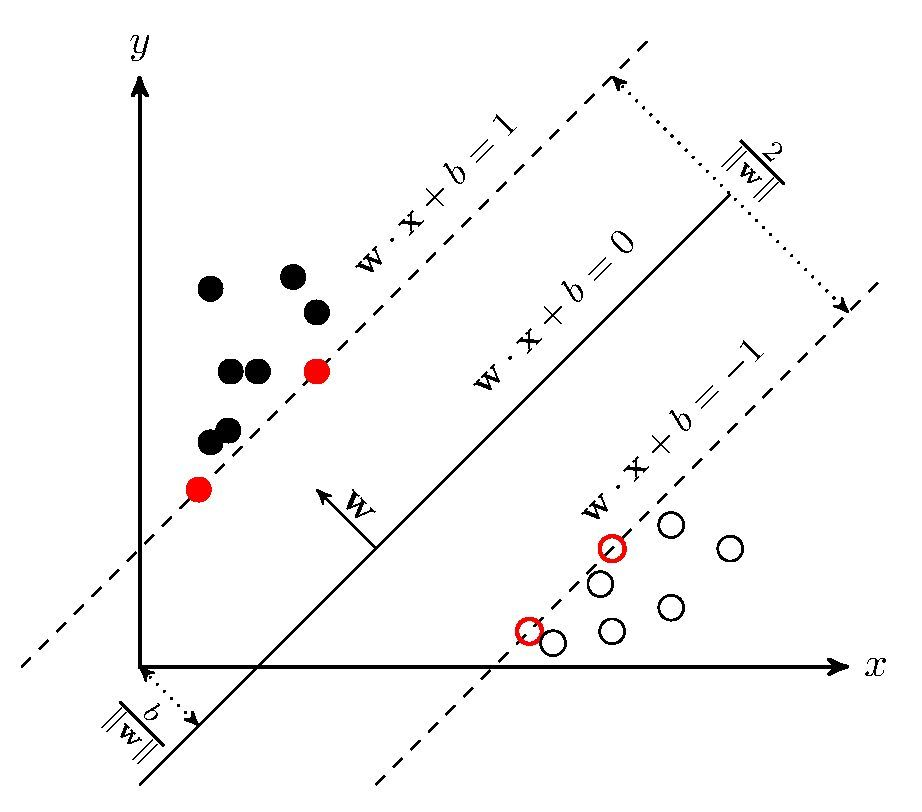
\includegraphics[width=\linewidth]{fig2}
  \caption{支持向量机示意图}
  \label{fig:svm}
  \vspace{-0.5cm}
\end{figure}

假设给定一个特征空间上的训练数据集 $T=\left\{\left(\boldsymbol{x}_1, y_1\right),\left(\boldsymbol{x}_2, y_2\right), \ldots,\left(\boldsymbol{x}_N, y_N\right)\right\}$,其中,$\boldsymbol{x}_i \in \mathbb{R}^n, \quad y_i \in\{+1,-1\}, i=1,2, \ldots N$, $x_i$ 为第 $i$ 个特征向量, $y_i$ 为类标记,当它等于+1时为正例;为-1时为负例。再假设训练数据集是线性可分的。对于给定的数据集 $T$和超平面 $\boldsymbol{w} \cdot x+b=0$,定义超平面关于样本点 $(x_i,y_i)$ 的几何间隔为

\begin{equation}
	\gamma_i=y_i\left(\frac{\boldsymbol{w}}{\|\boldsymbol{w}\|} \cdot \boldsymbol{x}_{\boldsymbol{i}}+\frac{b}{\|\boldsymbol{w}\|}\right)
\end{equation}


超平面关于所有样本点的几何间隔的最小值为

\begin{equation}
\gamma=\min _{i=1,2 \ldots, N} \gamma_i
\end{equation}

实际上这个距离就是我们所谓的支持向量到超平面的距离。根据以上定义,SVM模型的求解最大分割超平面问题可以表示为以下约束最优化问题

\begin{equation}
\begin{array}{ll}
\max _{\boldsymbol{w}, b} & \gamma \\
\text { s.t. } & y_i\left(\frac{\boldsymbol{w}}{\|\boldsymbol{w}\|} \cdot \boldsymbol{x}_{\boldsymbol{i}}+\frac{b}{\|\boldsymbol{w}\|}\right) \geq \gamma, i=1,2, \ldots, N
\end{array}
\end{equation}

将约束条件两边同时除以 $\gamma$,得到

\begin{equation}
y_i\left(\frac{\boldsymbol{w}}{\|\boldsymbol{w}\| \gamma} \cdot \boldsymbol{x}_{\boldsymbol{i}}+\frac{b}{\|\boldsymbol{w}\| \gamma}\right) \geq 1
\end{equation}

因为,$\|\boldsymbol{w}\|, \gamma$, 都是标量,所以为了表达式简洁起见,令

\begin{equation}
\begin{aligned}
&\boldsymbol{w}=\frac{\boldsymbol{w}}{\|\boldsymbol{w}\| \gamma} \\
&b=\frac{b}{\|\boldsymbol{w}\| \gamma}
\end{aligned}
\end{equation}

得到

\begin{equation}
y_i\left(\boldsymbol{w} \cdot \boldsymbol{x}_{\boldsymbol{i}}+b\right) \geq 1, i=1,2, \ldots, N
\end{equation}

又因为最大化 $\gamma$ 等价于最大化 $\frac{1}{\|\boldsymbol{w}\|}$,也就等价于最小化 $\frac{1}{2}\|\boldsymbol{w}\|^2$,因此SVM模型的求解最大分割超平面问题又可以表示为以下约束最优化问题

\begin{equation}
\begin{array}{ll}
\min _{\boldsymbol{w}, b} & \frac{1}{2}\|\boldsymbol{w}\|^2 \\
\text { s.t. } & y_i\left(\boldsymbol{w} \cdot \boldsymbol{x}_{\boldsymbol{i}}+b\right) \geq 1, i=1,2, \ldots, N
\end{array}
\end{equation}

这是一个含有不等式约束的凸二次规划问题,可以对其使用拉格朗日乘子法得到其对偶问题(dual problem),这里不再详细介绍。

\vspace{0.3cm}
\lstinputlisting[language=Python,firstline=108,lastline=110]{main.py}

同样可以利用 sklearn 包中提供的 Logistic 回归和 Adaboost 分类器来对数据进行训练。

\subsubsection{非极大值抑制}

除了目标表示和分类器的选择外,非极大值抑制也是目标检测算法中的重要环节。非极大值抑制(Non-Maximum Suppression,NMS),顾名思义就是抑制不是极大值的元素,可以 理解为局部最大搜索。这个局部代表的是一个邻域,邻域有两个参数可变,一是邻域的维数,二是邻域 的大小。例如在行人检测中,滑动窗口经提取特征,经分类器分类识别后,每个窗口都会得到一个分数。 但是滑动窗口会导致很多窗口与其他窗口存在包含或者大部分交叉的情况。这时就需要用到 NMS 来 选取那些邻域里分数最高(是行人的概率最大),并且抑制那些分数低的窗口。NMS 在计算机视觉领域 有着非常重要的应用,如视频目标跟踪、数据挖掘、3D 重建、目标识别以及纹理分析等。如图 \ref{fig:nms} 所示。

\begin{figure}[!ht]
  \centering
  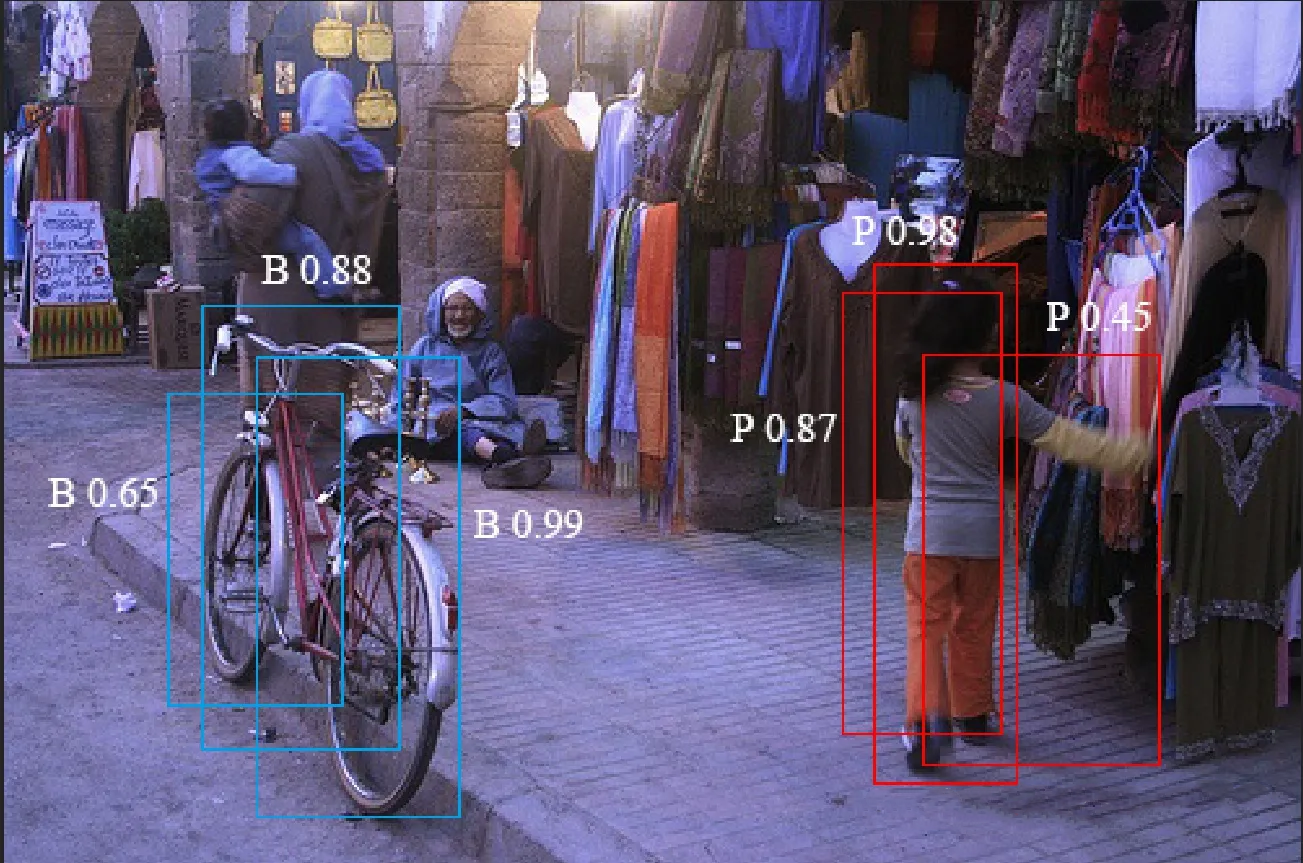
\includegraphics[width=0.5\linewidth]{fig3b}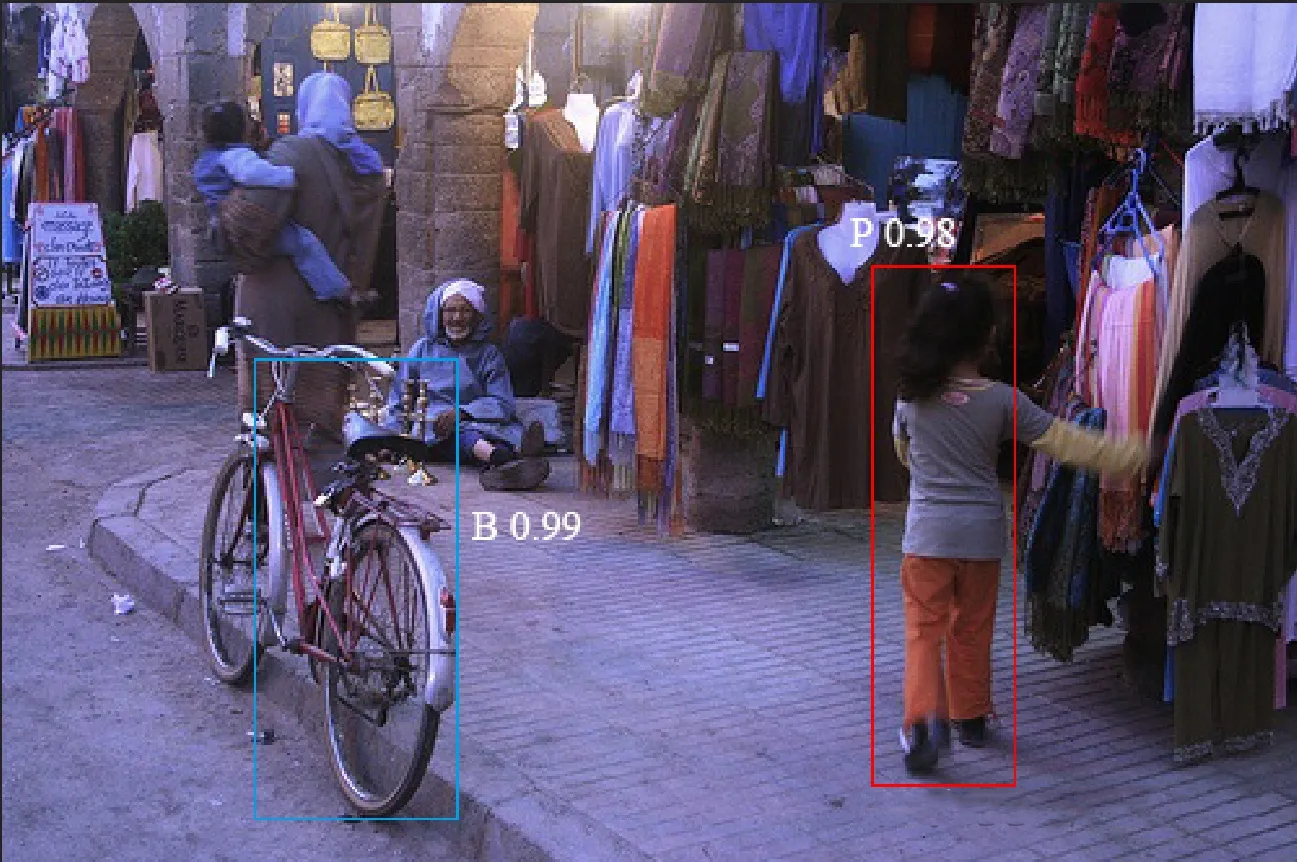
\includegraphics[width=0.5\linewidth]{fig3a}
  \caption{非极大值抑制示意图}
  \label{fig:nms}
\end{figure} 

本文所使用的非极大值抑制算法流程为:

\begin{enumerate}
	\item[(1)]将所有的框按类别划分,并剔除背景类,背景类无需 NMS;
	\item[(2)]对每个物体类中的边界框 (BBOX),按照分类置信度降序排列;
	\item[(3)]在某一类中,选择置信度最高的边界框 BBOX1,将 BBOX1 从输入列表中去除,并加入输出列表;
	\item[(4)]逐个计算 BBOX1 与其余 BBOX2 的交并比 IoU,若 IoU(BBOX1,BBOX2)> 阈值 TH,则在输入去除 BBOX2,IoU 计算公式为 $I O U=\frac{\text { 两边界框相交面积 }}{\text { 两边界框相并面积 }}$;
	\item[(5)]重复步骤(3) (4),直到输入列表为空,完成一个物体类的遍历;
	\item[(6)]重复步骤(2)(5),直到所有物体类的 NMS 处理完成。
	\item[(7)]输出列表,算法结束。
\end{enumerate}

代码实现如下:

\vspace{0.3cm}
\lstinputlisting[language=Python,firstline=54,lastline=87]{main.py}


\subsection{基于深度学习的口罩检测}

本文采用的用于口罩检测的神经网络为 Faster RCNN,经过R-CNN和Fast RCNN的积淀,Ross B. Girshick在2016年提出了新的Faster RCNN,在结构上,Faster RCNN已经将特征抽取(feature extraction),proposal提取,bounding box regression(rect refine),classification都整合在了一个网络中,使得综合性能有较大提高,在检测速度方面尤为明显。其网络结构如图 \ref{fig:faster-r-cnn} 所示:

\begin{figure}[!ht]
  \centering
  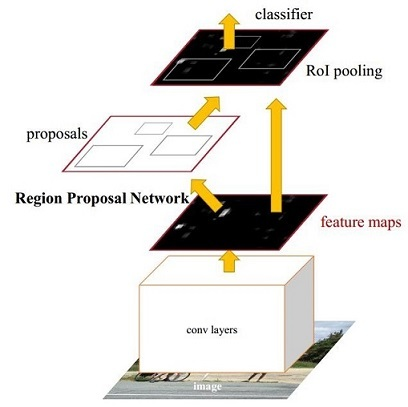
\includegraphics[width=\linewidth]{fig4}
  \caption{Faster RCNN 基本结构}
  \label{fig:faster-r-cnn}
\end{figure} 

\begin{enumerate}
	\item[(1)] Conv layers。作为一种CNN网络目标检测方法,Faster RCNN首先使用一组基础的conv+relu+pooling层提取image的feature maps。该feature maps被共享用于后续RPN层和全连接层;
	\item[(2)] Region Proposal Networks。RPN网络用于生成region proposals。该层通过softmax判断anchors属于positive或者negative,再利用bounding box regression修正anchors获得精确的proposals;
	\item[(3)] Roi Pooling。该层收集输入的feature maps和proposals,综合这些信息后提取proposal feature maps,送入后续全连接层判定目标类别;
	\item[(4)] Classification。利用proposal feature maps计算proposal的类别,同时再次bounding box regression获得检测框最终的精确位置。
\end{enumerate}

Faster R-CNN的训练,是在已经训练好的model(如VGG\_CNN\_M\_1024,VGG,ZF)的基础上继续进行训练。如图 \ref{fig:train} 所示,实际中训练过程分为6个步骤:

\begin{figure}[!ht]
  \centering
  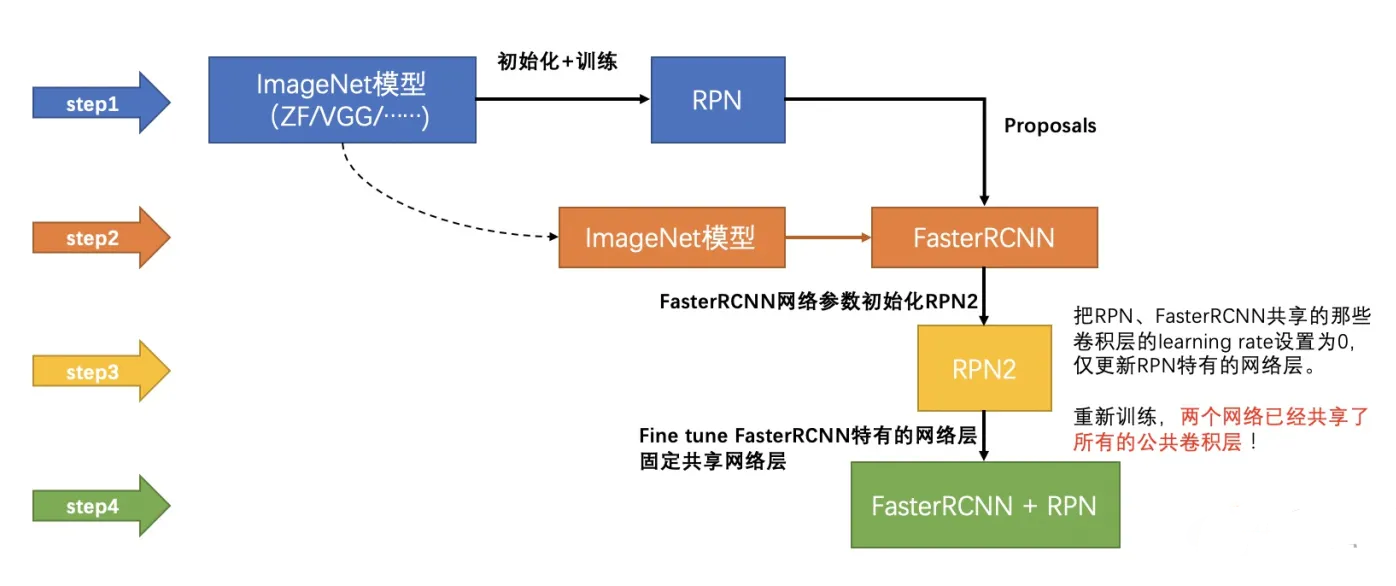
\includegraphics[width=\linewidth]{fig5}
  \caption{Faster RCNN 基本结构}
  \label{fig:train}
\end{figure} 

\begin{enumerate}
	\item[(1)] 在已经训练好的model上,训练RPN网络;
	\item[(2)] 利用步骤1中训练好的RPN网络,收集proposals;
	\item[(3)] 第一次训练Fast RCNN网络;
	\item[(4)] 第二训练RPN网络;
	\item[(5)] 再次利用步骤4中训练好的RPN网络,收集proposals;
	\item[(6)] 第二次训练Fast RCNN网络。
\end{enumerate}

本文利用 PyTorch 在 COCO 数据集上预训练的 Faster RCNN 模型,将模型预测器的输出维度调整为4(即佩戴口罩、未佩戴口罩、未正确佩戴口罩和背景),代码实现如下:

\vspace{0.3cm}
\lstinputlisting[language=Python,firstline=177,lastline=198]{main2.py}

数据集的构建和加载涉及图片数据的加载、标签文件的解析,代码实现如下:

\vspace{0.3cm}
\lstinputlisting[language=Python,firstline=201,lastline=326]{main2.py}

网络模型的训练代码实现如下\footnote{其余代码由于篇幅原因不再具体展示和说明。}:

\vspace{0.3cm}
\lstinputlisting[language=Python,firstline=334,lastline=356]{main2.py}